% !iTeXMac(input): POH.tex
\chapter{AIRPLANE HANDLING, SERVICE \& MAINTENANCE} \vspace{\minitocspacebefore} \minitoc \cleardoublepage

\section{INTRODUCTION} This is a place-holder for the Airplane Handling, Service \& Maintenance Section. The section will be completed once in-service experience has been gained.

\section{GROUND HANDLING}
Ground motion is best accomplished by pushing or pulling on the propeller as near to the
spinner as possible. The following are recommended aditional pushing locations to help move the
airplane: 

\begin{itemize*}
  \item Moving forward --- front seat support (canopy open).
  \item Moving rearwards --- wing leading edges and roots of horizontal stabilizer.
  \end{itemize*}

A suitable pushbar may be fitted over the two ends of the tailwheel axel.

Take care to not use high power during runup, as the tail will lift even if the control stick is held full aft.

Wing tie down mounting points are located centrally under each wing. Use a 3/8" dia x 16
tpi eyebolt to attach tie down rope to airplane. Secure a third line to the tail wheel spring.


\section{SERVICING}

\textcolor{red}{???}

\section{CLEANING AND CARE}

\textcolor{red}{???}

\section{COWLING REMOVAL} \textcolor{red}{See C-GFEW POH for example.}

\section{INSPECTION PANELS}
In addition to the engine cowling, the aircraft has a number of inspection and access panels:
\begin{enumerate*}
  \item Oil dipstick access door on aft right side of upper cowling.
  \item Instrument panel access door on aft wall of forward baggage compartment.  Four Torx T10 screws are removed, allowing the access panel to be opened.
  \item Three under-wing inspection panels on each wing provide access to fuel tank securing bolts and aileron bellcranks.
  \item Rear fuselage inspection plates on each side provide access to the elevator horns.
  \item Rear baggage compartment aft wall and hat shelf are removable, providing access to the battery and rear fuselage.
  \item Cockpit and rear baggage compartment floors are removable.
  \item Wing tips are removable, but note that they must remain close to the wing tips due to the coax connections to an internal antenna in each wing tip, and the power wires for the strobe and navigation lights in each wing tip.
  \end{enumerate*}


\section{INITIAL INSPECTIONS}

The following inspections are required following first flight:

\subsection{After First Flight} 
\begin{enumerate*}
	\item Complete firewall forward detailed visual inspection. 
	\item Check alternator belt tension (7--9 ft-lb on pulley when belt slips). 
	\item Complete airframe visual detailed inspection. 
\end{enumerate*}

%\subsection{2 Hours} 
%\begin{enumerate*}
%	\item Lubricate propeller hub. See 100 Hour Inspection or Hartzell Propeller Owner's Manual for details of procedure. 
%\end{enumerate*}

\subsection{10 Hours} 
\begin{enumerate*}
	\item Change oil, cut open oil filter and inspect, and inspect suction screen. Look for metal particles, shavings or flakes. Info from Lycoming Service Bulletin No. 480D, July 13, 2000. 
	\item Retorque landing gear bolts.
	\item Complete items from Conditional Inspection, except for oil change, propeller lubrication, ELT. 
\end{enumerate*}

\subsection{25 Hours} 
\begin{enumerate*}
	\item Check alternator belt tension (7--9 ft-lb on pulley when belt slips). 
\end{enumerate*}

\subsection{35 Hours} 
\begin{enumerate*}
	\item Change oil, cut open oil filter and inspect, and inspect suction screen. Look for metal particles, shavings or flakes. Info from Lycoming Service Bulletin No. 480D, July 13, 2000. 
	\item Complete items from Conditional Inspection, except for oil change, propeller lubrication, ELT. 
\end{enumerate*}

\section{PERIODIC MAINTENANCE} This section includes all items specified in the Lycoming Owner's Manual, MT Operation and Installation manual and Christen 801 Series Inverted Oil System Product Manual. \textcolor{red}{Add items from Slick mag service info.} It is supplemented by recommendations from Van's Aircraft, other RV owners, and engineering judgement.

\subsection{50 Hours or 4 months} The following items should be performed every 50 hours, or four months, whichever comes first:
\begin{enumerate*}
	\item Drain oil sump with oil hot. Send sample for analysis (see Lycoming Service Letter No. 171). 
	\item Replace oil filter. Cut open \& inspect. 
	\item Inspect \& clean suction oil screen. 
	\item Check \& record brake fluid level. 
	\item Check integrity of: 
	\begin{enumerate*}
		\item Fuel \& oil hoses, 
		\item Ignition system, 
		\item Magneto P-lead \& mounting bolts, 
		\item Exhaust system \& attachment hardware, 
		\item Cylinders - check for oil leak at rocker box covers, and check for signs of overheating (burned paint), 
		\item Baffling/plenum, 
		\item Firewall forward wiring, 
		\item Engine mount bolts, 
		\item Firewall seals, and 
		\item Cowling hinge eyes. 
	\end{enumerate*}
	\item Inspect \& lubricate: 
	\begin{enumerate*}
		\item Throttle, mixture \& prop linkages, 
		\item Alternate air door \& control, and 
		\item Oil cooler door \& control. 
		\item Tail wheel (disassemble, inspect locking pin for burrs, lubricate and reassemble) 
	\end{enumerate*}
	\item Check alternator belt condition \& tension. 
	\item Check tires for wear, rotate/replace as necessary. 
	\item On test flight, log engine data. 
\end{enumerate*}

\subsection{100 Hours or 12 months} The following items should be performed every 100 hours, or 12 months, whichever comes first: 
\begin{enumerate*}
	\item Complete the items from the 50 hour inspection, plus 
	\item Remove, clean, inspect and regap spark plugs.
	\item Inspect \& clean gascolator screen. 
	\item Inspect \& clean fuel filter. \textcolor{red}{Check recommended interval.} 
	\item Conduct compression check on all cylinders. 
	\item Propeller 
	\begin{enumerate*}
		\item Remove spinner 
		\item Inspect spinner and back plate. 
		\item Check propeller mounting bolts and safety wire. 
		\item Inspect prop blades for nicks and cracks. 
		\item Inspect prop hub for cracks or grease leakage. \textcolor{red}{Add any items from MT manuals}. 
		\item Check blade track. 
		\begin{enumerate*}
			\item Chock the wheels securely. 
			\item Place a fixed reference point beneath the propeller, within 0.25" below the lowest point of the propeller arc. Fasten a sheet of paper to the reference point. 
			\item Rotate the propeller by hand (opposite the direction of normal rotation) until a blade points directly at the paper. Mark the position of the blade tip on the paper. 
			\item Repeat the procedure with the second blade. 
			\item Tracking tolerance is 0.125" between the position of the two blades. 
		\end{enumerate*}
		\item Reinstall the spinner. 
	\end{enumerate*}
	\item Check alternator belt tension (7--9 ft-lb on pulley when belt slips). 
	\item Magneto
	\begin{enumerate*}
		\item Check breaker points for pitting and minimum gap, 
		\item Check for excessive oil in breaker compartment, 
		\item Lubricate breaker point felt, and 
		\item Check Magneto to Engine timing. See Lycoming Direct Drive Overhaul Manual for details of procedure.
	\end{enumerate*} 
	\item Electronic Ignition
	  \begin{enumerate*}
	    \item Remove Hall Effect Sensor and open up to check for gear, bearing and seal wear
	    \item Set electronic ignition timing
    	\end{enumerate*} 	
	\item Check cylinders visually for cracked or broken fins, 
	\item Check engine mounting bolts and bushings, 
	\item Check fuel injector nozzles for looseness, tighten to 60 in-lb torque, 
	\item Check fuel lines for dye stains at connections, and 
	\item Re-install spark plugs with new washers. 
\end{enumerate*}

\subsection{400 Hours} The following items should be performed every 400 hours: 
\begin{enumerate*}
	\item Replace spark plugs, and 
	\item Remove rocker box covers and check for freedom of valve rockers when valves are closed. Look for evidence of abnormal wear or broken parts in the area of valve tips, valve keeper, springs and spring seats. 
\end{enumerate*}

\subsection{500 Hours} 
\begin{enumerate*}
	\item\textcolor{red}{Insert Slick's recommended items.} 
	\item Electronic Ignition---the following items should be performed every 500 hours or 36 months: 
	\begin{enumerate*}
		\item Replace high tension leads (i.e. coil to spark plug wires), and 
		\item Remove cover from Hall effect module, and inspect for bearing wear or oil contamination. 
	\end{enumerate*}
\end{enumerate*}

\subsection{1500 Hours} The following items should be performed every 1500 hours or 10 years (from CAR 625 Appendix C --- not mandatory for amateur-built aircraft). MT's recommended overhaul interval is 1800 hrs or 72 months.
\begin{enumerate*}
	\item Overhaul propeller. 
\end{enumerate*}

\subsection{3 Months} The ELT Self Test must be performed every 3 months:
\begin{enumerate*}
	\item Battery Master Switch is OFF.
	\item ELT Switch is ARMED.
	\item Press Test/Reset Button on ELT Remote Control (right most button).
	\item ELT Remote Control Lamp should flash once.
	\item A single beep will sound if the ELT passes the self test.
	\item Two to Five beeps will sound if there is a problem:
	\begin{enumerate*}
	  \item 2 beeps, followed by 2 second delay, followed by 2 beeps: battery low.
	  \item 3 beeps, followed by 2 second delay, followed by 3 beeps: low RF power.
	  \end{enumerate*}
\end{enumerate*}

\subsection{12 Months} The following items must be performed every 12 months:
\begin{enumerate*}
	\item Conduct compass swing of any non-stabilized magnetic compass and install dated compass card (requirement from CAR 625 Appendix C).
	\item Inspect ELT (requirement from CAR 625 Appendix C).
\end{enumerate*}

\subsection{24 Months} The following items must be performed every 24 months:
\begin{enumerate*}
	\item Calibrate altimeter and altitude encoder IAW AWM 571 Appendix B (requirement from CAR 625 Appendix C).
	\item Test transponder IAW AWM 571 Appendix F (requirement from CAR 625 Appendix C).
\end{enumerate*}

\section{ANNUAL INSPECTION} An annual inspection must be carried out once every 12 months.  The inspection must include all items listed in CAR 625 Appendix B.  The following list expands on the required items.  Items marked with (*) are not required as per CAR 625 Appendix B.  Completion of these items is not required as per the CARs, but is strongly recommended to improve reliability and safety.

\begin{enumerate*}
  \item{Aircraft General}
  \begin{enumerate*}
    \item Remove or open all inspection panels, access doors, fairings and cowlings.
    \item Thoroughly clean the aircraft.
    \item Inspect panel, door and cowling closing and locking mechanisms for improper installation, function and condition.
		\end{enumerate*}

	\item{Fuel System} 
	\begin{enumerate*}
		\item Fuel Filter --- clean and inspect. 
		\item Gascolator --- clean and inspect. 
		\item Fuel Lines --- inspect.
		\item Leaks --- check fuel system for leaks.
		\item Fuel Pressure --- Check pressure from electric fuel pump is 25--45 psi. 
		\item Fuel Selector Valve --- inspect and check operation.
		\item Fuel Vents --- inspect.
	\end{enumerate*}


	\item{Engine} 
	\begin{Note}
		[WARNING] \centering Ground mags before working on engine. 
	\end{Note}
	\begin{enumerate*}
		\item Remove engine cowl.
		\item Cowling --- clean it and inspect for cracks, distortion and loose or missing fasteners.
		\item Leaks --- inspect engine, oil lines, oil cooler and inverted oil system for oil leaks.
		\item Oil 
		\begin{enumerate*}
			\item Oil temp. sender --- inspect for leaks and security. 
			\item Oil lines and fittings --- inspect for leaks, chafing security, dents and cracks. 
			\item Oil cooler --- clean cooling fins and inspect condition.  (*)
			\item Inverted oil system --- inspect for for leaks and security. 
			\item Screens and sump drain plugs --- inspect for metal particles and foreign matter.
			\item Fill engine with oil per \textcolor{red}{lubrication chart}. 
		\end{enumerate*}
		\item Ignition (*)
		\begin{enumerate*}
			\item Check condition of spark plugs and adjust gap. 
			\item Check ignition harness and insulators. 
			\item Check magneto points for proper clearance maintain at \textcolor{red}{.018 $\pm $ .006}. 
			\item Check magneto for oil seal leaks. 
			\item Check breaker felt for proper lubrication. 
			\item Check distributor block for cracks, burned areas or corrosion. 
			\item Check magnetos to engine timing. See Lycoming Direct Drive Overhaul Manual for details of procedure. 
			\item Check electronic ignition timing
		\end{enumerate*}
		\item Thoroughly clean engine and other items ahead of the firewall.
		\item Studs and nuts --- inspect for defects, evidence of improper torque and safety locking.
  	\item Cylinder compression --- conduct compression check on all cylinders.  Record readings.  If compression test indicates problems, check internal condition and tolerances.
		\item Remove air filter and clean. 
		\item Check condition of alternate air door and cable.
		\item \textcolor{red}{Bendix FI items??} 
		\item Clean screens in fuel pump. 
		\item General condition:
		\begin{enumerate*}
		\item Check engine controls throttle, carb heat, mixture, prop and alternate air door.  Check condition, proper travel and safety locking.
		\item Exhaust system --- inspect for cracks, defects and improper attachment.
		\item Inspect heater muffs, heater boxes and SCAT tubes.
		\item Check breather tube for obstructions and security.
		\item Check crankcase for cracks, leaks, security of bolts.
		\item Engine mounts --- inspect for cracks, looseness of mounting and looseness of engine to mount
		\item Flexible vibration dampeners --- inspect for poor condition and deterioration.
		\item Check all engine baffles and plenum parts.
		\item Check firewall seals.
		\item Check condition and tension of alternator, alternator mount, drive belt and B-lead.
		\item Check condition of starter, starter mount, starter cable and solenoid.
		\item Check standby alternator.
		\item Check prop governor.
		\item Internal corrosion --- inspect engines which have not been inhibited and have been out of service in excess of 12 months.
	  \end{enumerate*}
		\item Check \& record brake fluid level.  (*)
		\item Lubricate all controls.
		\item Reinstall engine cowl. 
	\end{enumerate*}
	\item{Fuel System} 
	\begin{enumerate*}
		\item Clean and inspect fuel filter. 
		\item Clean and inspect gascolator. 
		\item Inspect condition of fuel lines.
		\item Check fuel system for leaks.
		\item Check pressure from electric fuel pump is 25--45 psi. 
		\item Check operation of fuel selector valve.
		\item Check fuel vents.
	\end{enumerate*}

	\item{Propeller} 
	\begin{enumerate*}
	  \item Propeller hub assembly --- inspect for cracks, nicks, binding and oil leakage.
	  \item Bolts and nuts --- inspect for improper torque and safety locking.
	  \item Control mechanisms --- inspect for improper operation, insecure mounting and improper range of travel.
	  \item Composite blades --- inspect for:
	  \begin{enumerate*}
	    \item cracks, bruises, scars, warping, evidence of glue failure and delamination,
	    \item attachment bolt tightness, and
	    \item correct track, excessive rotational and end play.

  	  \end{enumerate*}
  	\item Spinner assembly --- inspect for cracks and wear.
  	\item Variable pitch propellers --- check correct operation during ground run.
	\end{enumerate*}


	\item{Cockpit} 
	\begin{enumerate*}
		\item Remove seats and cockpit floors. 
		\item Generally --- inspect for dirt and loose equipment that might foul the controls.
		\item Inspect cockpit area, forward fuselage and underfloor area for corrosion, cracks, chafed wiring, deterioration, distortion, evidence of failure, defective or insecure attachment fittings, etc. 
		\item Check for dirt and loose equipment that might foul the controls.
		\item Check all wing front spar attachment bolts.
		\item Check rear spar carry through structure.
		\item Inspect COM 1 and transponder antennae and coax.
		\item Landing gear boxes --- inspect condition of wiring, etc.  Check for FOD.
		\item Landing gear attach bolts --- Check torque (\textcolor{red}{add torque values}). 
		\item Controls:
  	\begin{enumerate*}
  		\item Check control columns, systems and connection.
  		\item Lubricate control column bearings as required.
  		\item Check pitch and roll trim operation from front and rear seats. 
  		\item Check flap motor, wiring and pushrods.
  		\item Lubricate flap pushrod bearings as required.
  	  \end{enumerate*}
		\item Reinstall cockpit floors and front seat. 
		\item Windscreen and canopy --- inspect for deterioration and breakage.
		\item Windscreen and canopy --- inspect canopy tracks, rollers and latch.
		\item Upholstery --- inspect for security and tears. (*)
		\item Seats and safety belts --- inspect for poor condition, fraying, and any other apparent defects.
		\item Rudder pedals, brake cylinders, parking brake valve and brake lines --- check condition.
		\item Gooseneck and instrument lights --- check condition and function of lamps and dimmers.
		\item Instrument Panel:
  	\begin{enumerate*}
  		\item Instruments --- inspect for poor condition, mounting, marking and, where practicable, for improper operation.
  		\item Placards ---- confirm all placards listed in the POH are in place and are legible.
  		\item Static System --- conduct static system leak check. (*)
      \end{enumerate*}
		\item Check condition of heater controls.
		\item Check condition of throttle, mixture and propeller speed controls.
		\item Check condition of oil cooler door and alternate air controls.
		\item Check condition and operation of air vents.
		\item Check fire extinguisher.
		\item Check wire bundles for chafing, paying particular attention to Infinity stick grip wire bundle at bottom of stick.
	\end{enumerate*}
	\item{Aft Fuselage} 
	\begin{enumerate*}
		\item Remove aft baggage floor and aft baggage rear bulkhead. 
		\item Check under whole aft fuselage, including skins, bulkheads, longerons, stiffeners ,under baggage floor area for corrosion, cracks, chafed wiring, deterioration, distortion, evidence of failure, defective or insecure attachment fittings, etc.
		\item Battery --- inspect for improper installation and improper charge.  Inspect battery hold-down and battery cables.  Check battery voltage with no load.
		\item Strobe power supply --- Check condition and wiring.
		\item GPS antenna --- check condition of antenna and coax cable.
		\item Elevator bellcrank and elevator control tubes --- check condition.  Lubricate bellcrank and pushrod ends as required. 
		\item Reinstall aft baggage floor and aft baggage rear bulkhead. 
	\end{enumerate*}
  \item{ELT} 
  \begin{enumerate*}
  	\item Inspect mounting tray and fasteners. 
  	\item Inspect coax cable for abrasion. Disconnect coax connections and inspect jack and plug for corrosion. 
  	\item Inspect cable to remote control for abrasion. Disconnect connections and inspect for corrosion. 
  	\item Inspect GPS data cable for abrasion. Disconnect GPS data cable and inspect jack and plug for corrosion.
  	\item Check expiration date of ELT, aural alert and remote batteries and replace if they will expire within the next 12 months. 
  	\item Conduct g-switch test from FAA Order 8250.3. From ACK manual, page 15. (*)
  	\begin{enumerate*}
  		\item Remove ELT from tray. 
  		\item Select ELT switch to ARMED. 
  		\item Monitor 121.5, with squelch turned OFF. 
  		\item During first five minutes of the hour, test g-switch: 
  		\begin{enumerate*}
  		  \item hold the ELT at your waist with the arrow printed on the battery case facing away from you. 
  		  \item move the ELT rapidly away from your waist. 
  		  \item when the ELT reaches the full extent of your arm retract it back to your waist as fast as possible.
  		  \end{enumerate*} 
  		\item Verify that the ELT tone is heard. 
  		\item Select ELT switch to OFF within 30 s (406 MHz emergency signal is sent 50 s after g-switch activation). 
  	\end{enumerate*}
  	\item Reinstall ELT
  	\item Set ELT switch to ARMED
  	\item Replace red guard over ELT switch
  	\item Reseal DIN connector with tape
  	\item Perform ELT Self Test, due every three months
  \end{enumerate*}
	\item{Empennage} 
	\begin{enumerate*}
		\item Remove empennage fairing and elevator horn inspection covers. 
		\item Check horizontal stabilizer attachment. 
		\item Check vertical fin attachments. 
		\item Check vertical fin and rudder surfaces. 
		\item Check rudder horn and attachment. 
		\item Check rudder bolts for wear. 
		\item Check rudder strobe and nav light for security. 
		\item Check horizontal stabilizer and elevators. 
		\item Check elevator trim tab and servo. 
		\item Check elevator horn. 
		\item Check elevator bolts for wear. 
		\item Lubricate all bearings as needed. 
		\item Reinstall empennage fairing and elevator horn inspection covers. 
	\end{enumerate*}
	\item{Wings} 
	\begin{enumerate*}
		\item Remove wing root fairing and under-wing inspection panels. 
		\item Check fuel tank to fuselage mount.
		\item Check wing rear spar attachment bolts.
		\item Check surfaces for damage and loose rivets. 
		\item Check wing walk condition.
		\item Check flaps and pushrods.
		\item Check fuel tank bolts on front spar.
		\item Check aileron bellcrank and control tubes.
		\item Lubricate aileron bellcrank and pushrods as required.
		\item Check aileron mounts and attachments.
		\item Lubricate aileron hinges as required.
		\item Check landing and taxi lights and lenses - condition and function.
		\item Check nav lights and strobes - condition and function.
		\item Check wing tips.
		\item Remove wing tips and inspect internal antennae.
		\item Reinstall wing root fairing and under-wing inspection panels. 
	\end{enumerate*}
	\item{Wheels and Brakes} 
	\begin{enumerate*}
		\item Tail wheel assembly. 
		\begin{enumerate*}
		  \item Tail wheel pivot --- disassemble.
		  \item Tail wheel pivot and locking mechanism --- inspect and lubricate.
		  \item Tail wheel axle --- disassemble.
		  \item Tail wheel bearings --- inspect and lubricate.
		  \item Tail wheel axle and tail wheel assembly --- reassemble and reinstall on aircraft
	  \end{enumerate*}
		\item Wheel pants and gear leg fairings --- remove. 
		\item Wheels --- remove.
		\item Wheels --- inspect for cracks, corrosion, defects broken bolts and condition of bearings.
		\item Wheel bearings --- clean, inspect and repack.
		\item Tires - inspect for wear, cuts and incorrect inflation; inspect for improper installation and improper operation.  Rotate as required.
		\item Brake lining and disc --- inspect.
		\item Landing gear legs --- inspect.
		\item Wheels --- reinstall. 
		\item Brake lines --- inspect for leaks and condition.
		\item Landing gear wear plate at lower fuselage longeron --- inspect.
		\item Wheel pants, gear leg fairings and intersection fairings ---  inspect.
		\item Wheel pants and gear leg fairings --- reinstall. 
	\end{enumerate*}
	\item{Operational Inspection} 
	\begin{enumerate*}
		\item Check items that wouldn't normally be checked in flight. \textcolor{red}{Which items??} 
	\end{enumerate*}
	\item{Engine Ground Run}
	\begin{enumerate*}
		\item Idle and maximum rpm --- check (for safety reasons, the check of maximum rpm will be done during a takeoff, rather than during a ground run).
		\item Magneto drop --- check.
		\item Oil and fuel pressures --- check.
		\item Cylinder and oil temperatures --- check.
		\item Propeller governor operation -- check.
		\item Standby Alternator operation -- check.
	\end{enumerate*}

\end{enumerate*}

\section{ALTERNATOR BELT TENSION} 
\begin{enumerate*}
	\item Adjust tension arm so that 11--13 ft-lb (new alternator belt), or 7--9 ft-lb (used alternator belt) of torque on the alternator pulley is required to slip the pulley on the alternator belt (from Lycoming SI 1129A Accessory Drive Belt Tension). 
	\item See Torque Table for tension arm and pivot bolt torque values. 
\end{enumerate*}

\section{MAGNETO TIMING} 
\begin{enumerate*}
	\item See the Lycoming Direct Drive Overhaul Manual for the detailed procedure. 
	\item Mag timing box --- Connect the black lead to the ground screw on the magneto.  Connect the red or green lead to the mag lead screw.  The red and green lamps on the timing box work backwards to what is described in the overhaul manual - the lamps extinguish when the points open, i.e. when the ignition fires. 
	\item The Mag Switch must be ON to use the timing box. 
	\item This serial number engine has a timing setting of 20\textdegree ~BTDC. 
	
\end{enumerate*}

\section{ELECTRONIC IGNITION}
\subsection{IGNITION TIMING} 
\begin{enumerate*}
	\item See the Lightspeed Engineering Plasma II Manual for the detailed timing procedure. 
	\item Set the engine to 5\textdegree ~after TDC for cylinders 1 and 2.
	\item Disconnect the two coax at the LightSpeed box.
	\item Select the EI Switch to ON.
	\item Rotate the hall effect module CCW until the green LED goes ON, then OFF.  Torque the hall effect module in place.
\end{enumerate*}
  \subsection{PHASE CHECK} 
  \begin{enumerate*}
  	\item disconnect all spark plug wires at the coils.  
  	\item Select EI Switch to ON.  
  	\item Set prop to 5\textdegree ~after TDC for cylinders 1 and 2.  
  	\item Briskly rock prop back and forth --- look for a spark at the spark plug lead connections on one of the coils.  
  	\item Connect the spark plug leads for cylinders 1 and 2 to the coil that produced the spark.
\end{enumerate*}

\section{SPARK PLUG GAPS}
Automotive spark plug, upper plugs, fired by electronic ignition - 0.026"--0.035" gap.

Aviation spark plug, lower plugs, fired by magneto - 0.016"--0.021" gap.

\section{PROPELLER GOVERNOR}
One CW turn of high rpm adjustment screw should decrease max speed by 25 RPM. 

\section{RETORQUE MAIN LANDING GEAR BOLTS}
  \begin{enumerate*}
    \item Torque the 7/16" bolts on the outboard end of each main landing gear leg with the torque wrench on the nut below the aircraft.  Hold the bolt heads with a 1/4" drive socket on a ratchet. 
    \item Torque the 7/16" bolt on the inboard end of each gear leg with the torque wrench on the nut inside the cockpit.  
    \item Torque the two 5/16" bolts at the inboard end of each gear leg with the torque wrench on the bolt head below the aircraft.  Hold the nuts with a 1/2" open end wrench.  
\end{enumerate*}

\section{TORQUE TABLE} 
\begin{tabularx}
	{
	\textwidth}{|>{\setlength\hsize{.9\hsize}}Y|c|>{\setlength\hsize{1.1\hsize}}Y|} \hline Item&Torque Value&Remarks\\
	\hline \hline Main Alternator Mount&110--150 in-lb&from Installation Instructions\\
	\hline Main Alternator Tension Arm&110--150 in-lb&from Installation Instructions\\
	\hline Main Alternator Pivot Bolt&30--40 ft-lb&from Installation Instructions\\
	\hline Spark Plugs (Aviation)&35 ft-lb&from Lycoming\\
	\hline Spark Plugs (Automotive)&180 in-lb&from Electronic Ignition Installation Instructions\\
	\hline Spark Plug Adaptors&25 ft-lb&Do no apply anti-seize.  from Electronic Ignition Installation Instructions\\
	\hline Magneto and EI Hall Effect Unit Base Clamps&204 in-lb&from ECI Service Info\\
	\hline Propeller Governor Mounting Nuts&110--150 in-lb&from PCU-5000 Installation and Adjustment document\\
	\hline Propeller Governor High RPM Stop Jam Nut&24.8--28.3 in-lb&from PCU-5000 Installation and Adjustment document\\
	\hline Propeller Hub&63--66 ft-lb&from MT Operation and Installation manual\\
	\hline Spinner Screws&35--44 in-lb&from MT Operation and Installation manual\\
	\hline Brake caliper bolts&90 in-lb&from Cleveland service info\\
	\hline Wheel half bolts&90 in-lb&Bolts that join the two halves of each wheel. Value from Cleveland service info\\
	\hline Landing gear outboard 7/16" bolts&240 in-lb&from RV-8 Builder's Manual\\
	\hline Landing gear inboard 7/16" bolts&450 -- 500 in-lb&from AC43.13-1B\\
	\hline Landing gear inboard 5/16" bolts&100 -- 140 in-lb&from AC43.13-1B\\
	\hline 
\end{tabularx}

\clearpage
\section{FUSE BLOCKS}
\begin{figure}
  \centering
  % 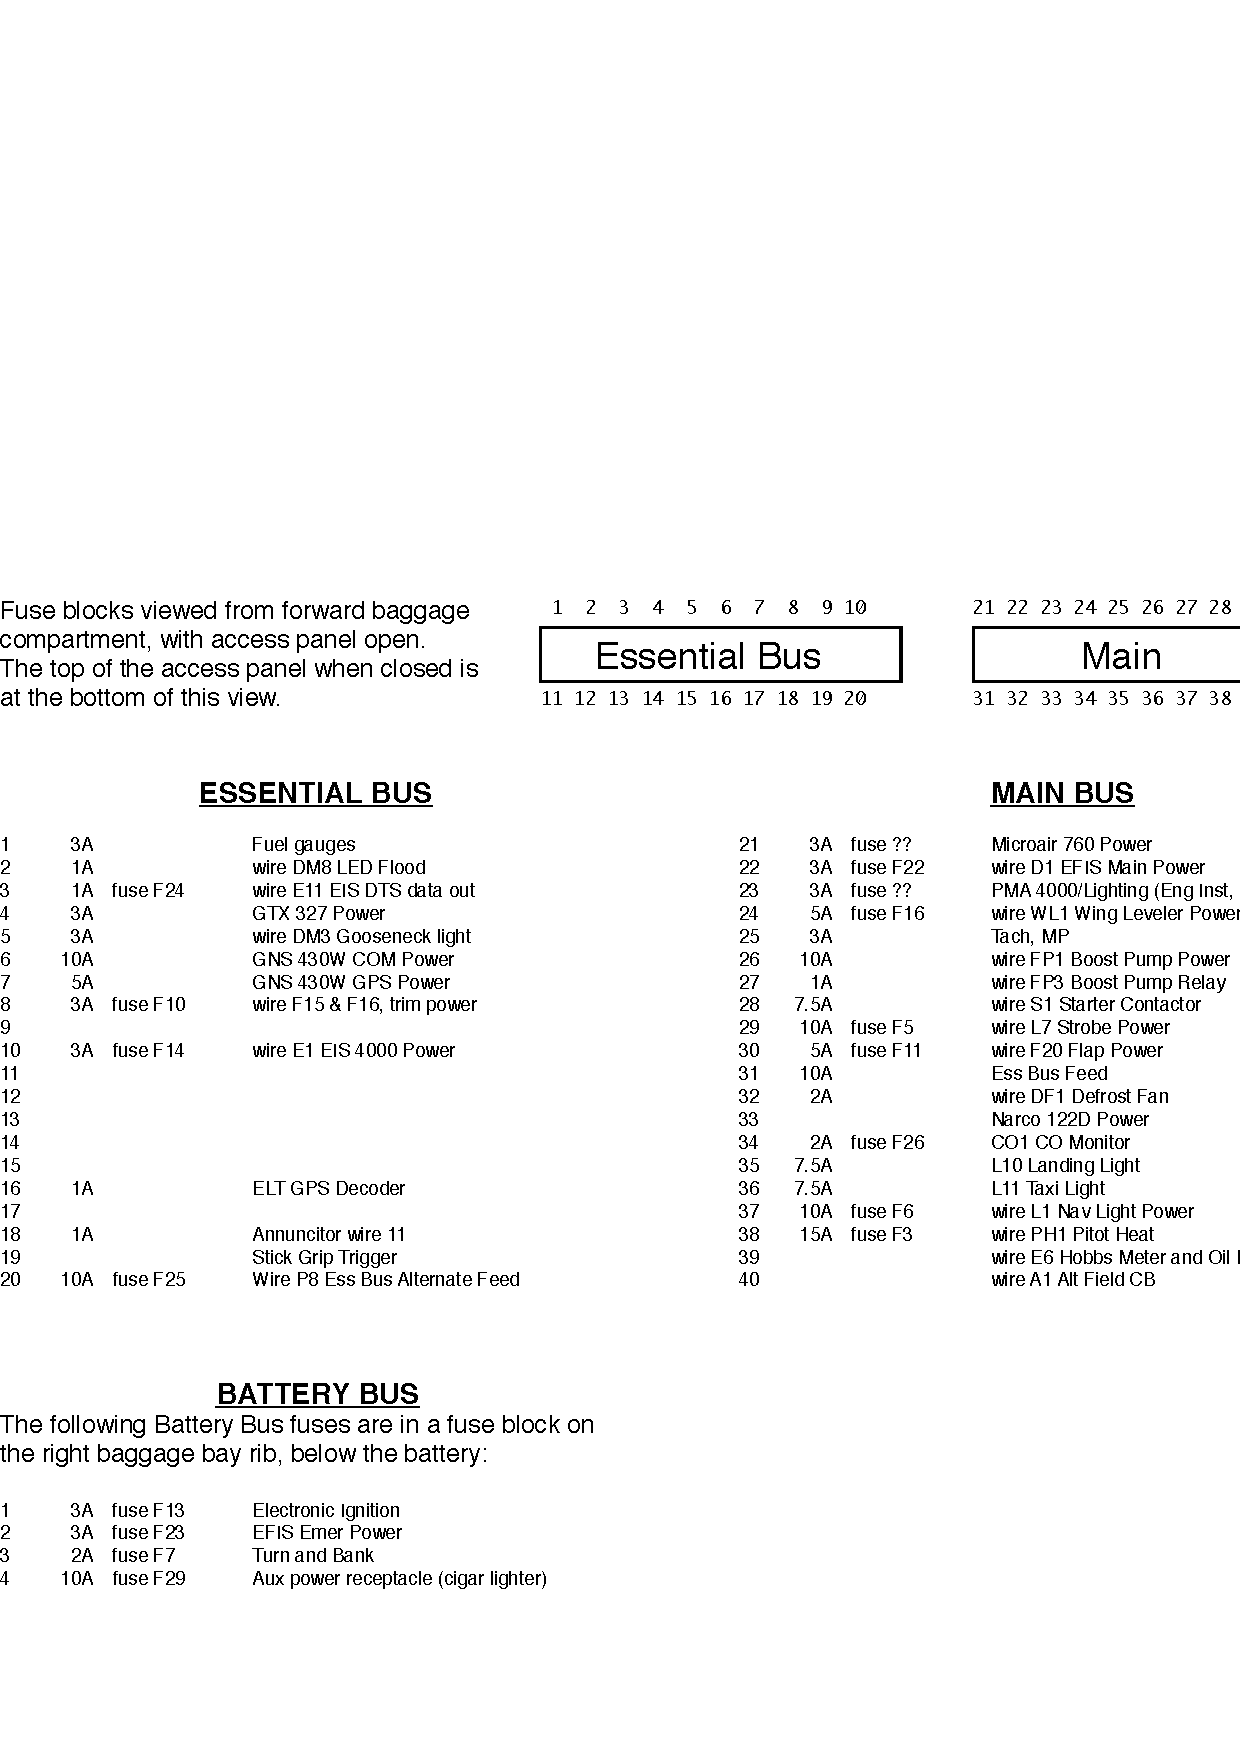
\includegraphics[width=1.1\textwidth, angle=90]{../Diagrams/Fuse_Blocks_POH}
  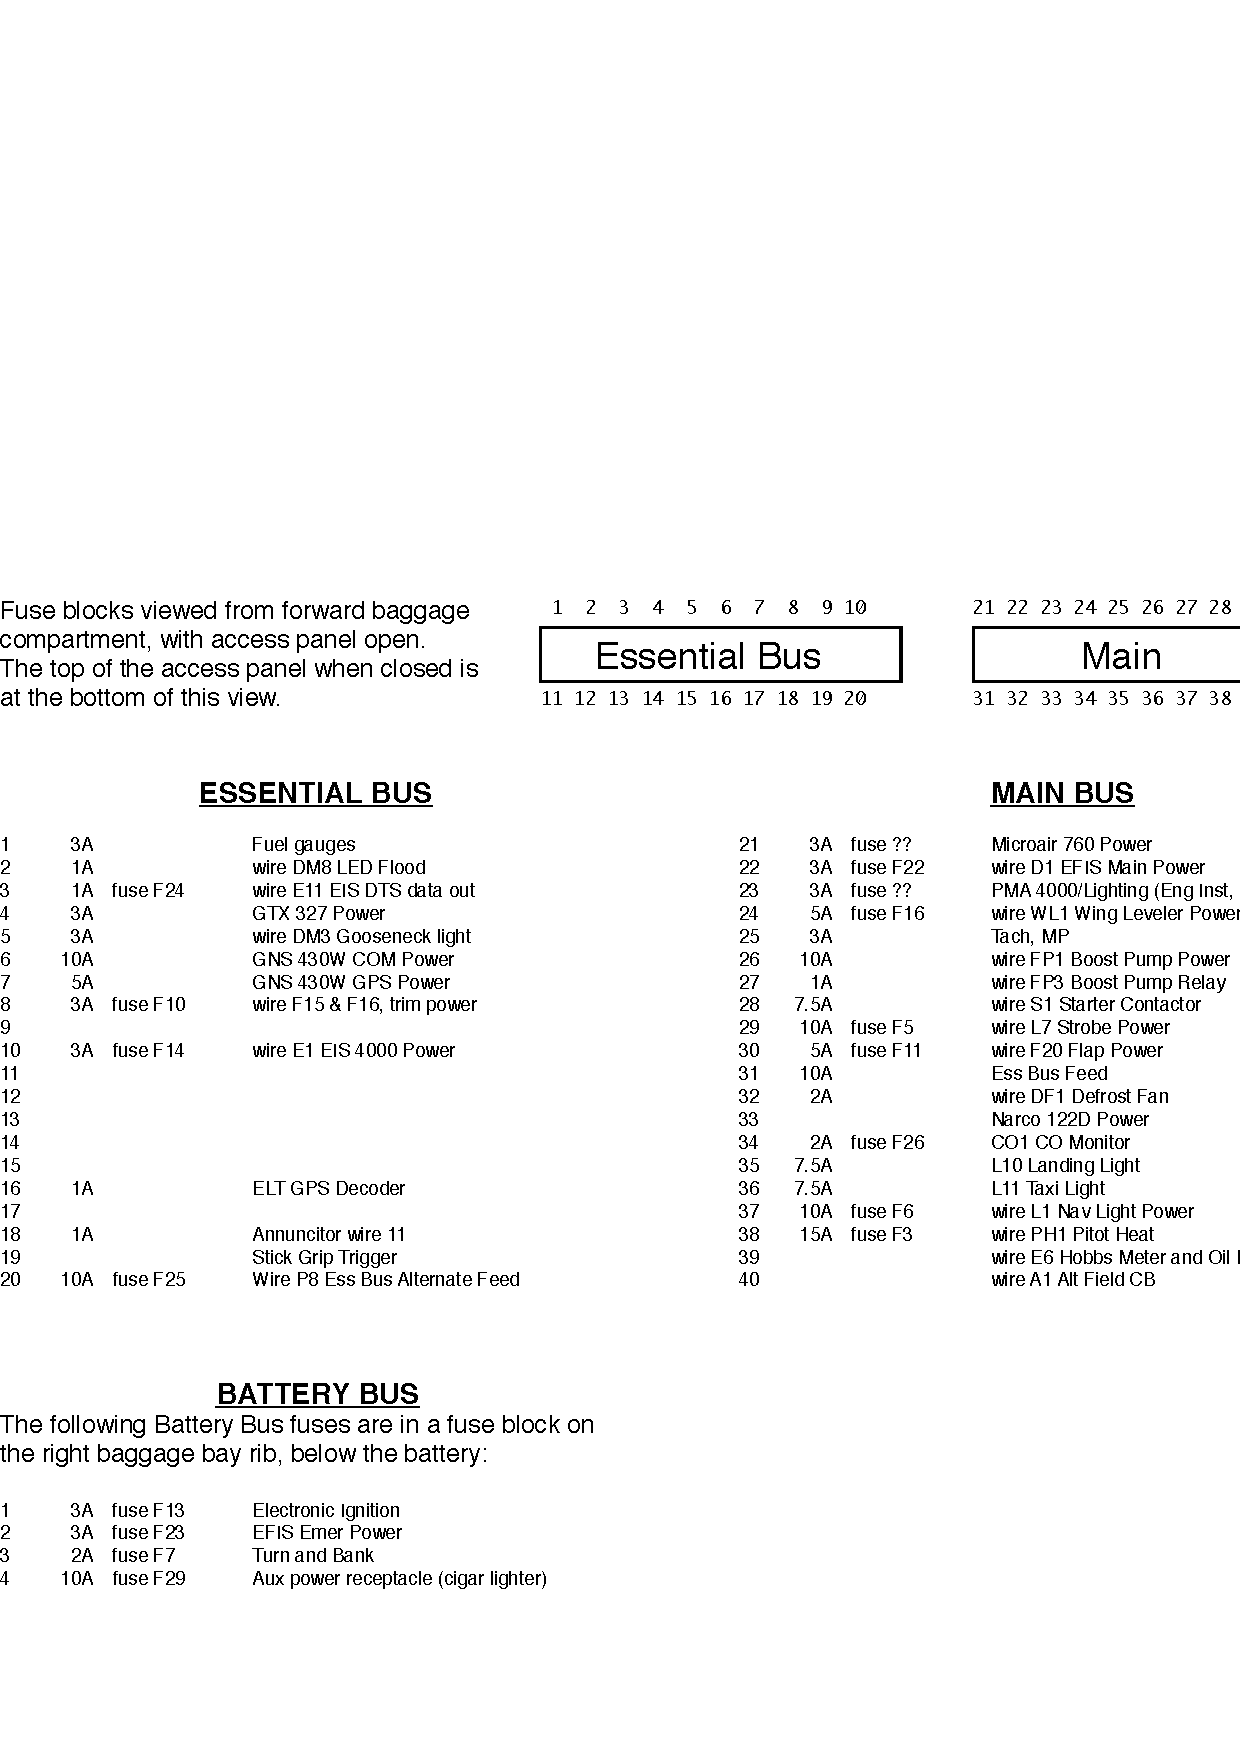
\includegraphics[width=1.2\textwidth, angle=90]{../Diagrams/Fuse_Blocks_POH}
  \label{fig:FuseBlocks}
  \caption{Fuse Blocks}
\end{figure}
\cleardoublepage 
